%% =====================================================================
\section{Results}
\label{sec:results}

\subsection{Study I: learning, controls and the mediator}
\label{sec:resI}
Table~\ref{tab:primary} lists the confirmatory verdicts of Study~I and Fig.~\ref{fig:forest} all contrasts.

% generated by scripts/paper_assets.py -- do not edit
\begin{table*}[t]
\centering
\caption{Confirmatory contrasts (pre-registered L1--L4). Sig.\ (A/C): number of instances significant after Holm in favour of the anchor / comparator. $\bar W$: mean paired win probability of the anchor with 95\% bootstrap CI. Rel.\ diff.: median over instances of the median paired relative difference (comparator$-$anchor)/$|$comparator$|$ (positive: anchor lower; descriptive, not pre-registered). Verdicts by the frozen decision rule.}
\label{tab:primary}
\footnotesize
\setlength{\tabcolsep}{4pt}
\resizebox{\textwidth}{!}{%
\begin{tabular}{llllrccccl}
\toprule
 & Domain & Anchor & Comparator & $n$ & Sig.\ (A/C) & $\bar W$ & 95\% CI & Rel.\ diff. & Verdict \\
\midrule
L1 & CEC2022 & SARSA & RND-FAIR & 100 & 0/1 & 0.461 & [0.434, 0.489] & $-4.3{\times}10^{-4}$ & comparator \\
L1 & FIR & SARSA & RND-FAIR & 100 & 0/1 & 0.443 & [0.409, 0.476] & $-1.1{\times}10^{-2}$ & comparator \\
L2a & CEC2022 & RND-SYNC & RND-REEVAL & 50 & 0/0 & 0.534 & [0.495, 0.573] & $6.3{\times}10^{-12}$ & inconclusive \\
L2a & FIR & RND-FAIR & RND-REEVAL & 50 & 1/0 & 0.575 & [0.527, 0.623] & $1.4{\times}10^{-2}$ & anchor \\
L2b & CEC2022 & RND-FAIR & RND-SYNC & 50 & 9/2 & 0.717 & [0.690, 0.743] & $1.9{\times}10^{-1}$ & mixed \\
L3 & CEC2022 & SARSA & SKEL & 50 & 4/2 & 0.579 & [0.545, 0.613] & $1.0{\times}10^{-9}$ & mixed \\
L3 & FIR & SARSA & SKEL & 50 & 8/0 & 0.962 & [0.943, 0.980] & $5.4{\times}10^{-1}$ & anchor \\
L4 & CEC2022 & SKEL & MPHB & 50 & 12/0 & 0.780 & [0.757, 0.802] & $6.4{\times}10^{-11}$ & anchor \\
L4 & FIR & SKEL & MPHB & 50 & 8/0 & 0.826 & [0.798, 0.853] & $1.3{\times}10^{-8}$ & anchor \\
\bottomrule
\end{tabular}}
\end{table*}


\begin{figure}[!htbp]
\centering
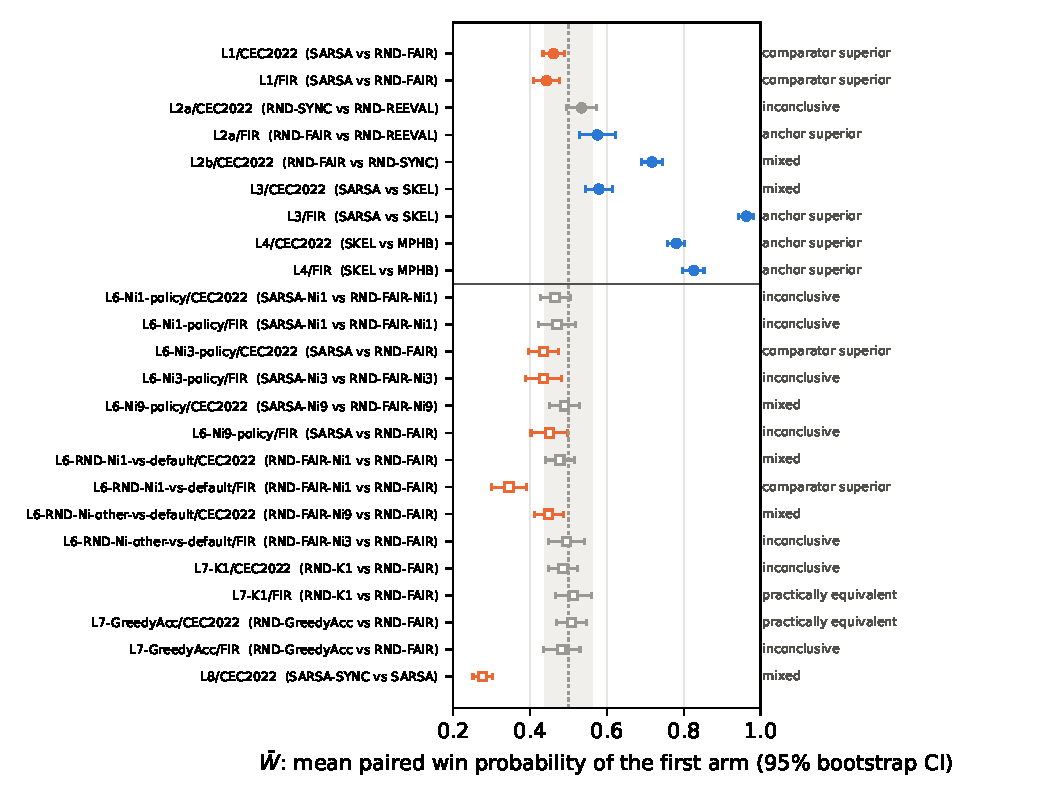
\includegraphics[width=0.78\textwidth]{figures/fig_forest.pdf}
\caption{Study I: mean paired win probability $\bar W$ of the first arm with 95\% bootstrap interval for every contrast
(circles: confirmatory; squares: exploratory; blue/orange: interval above/below 0.5). The shaded band is the
negligible-effect band of the decision rule.}
\label{fig:forest}
\end{figure}

\paragraph{Learning (L1)} At equal budget, SARSA does not outperform random assembly on either benchmark. On CEC2022 its mean
paired win probability is \res{A-H1-CEC2022-wbar} \res{A-H1-CEC2022-ci} and on FIR \res{A-H1-FIR-wbar} \res{A-H1-FIR-ci}. Both
intervals lie below 0.5, one instance per benchmark is significant in favour of the random mediator, and none favours SARSA,
so the pre-registered verdict is \emph{comparator superior} on both. The effect is small: the median relative difference is
$\res{A-H1-CEC2022-rel}$ on CEC2022 and $\res{A-H1-FIR-rel}$ on FIR (negative: SARSA's error is higher).

\paragraph{The re-evaluating control (L2)} With the memory update held fixed, the extra FEs of the control do not produce a
conclusive difference on CEC2022 ($\bar W=\res{A-H2a-CEC2022-wbar}$ \res{A-H2a-CEC2022-ci}, \emph{inconclusive}). On FIR,
where by Proposition~\ref{prop:memory} the extra block affects only the budget, the budget-identical random mediator is better
than the control ($\bar W=\res{A-H2a-FIR-wbar}$ \res{A-H2a-FIR-ci}, \emph{anchor superior}). The memory update has a large
effect on CEC2022 (L2b): random assembly \emph{without} the update beats the same mediator with it on \res{A-H2b-CEC2022-siga}
of 12 functions ($\bar W=\res{A-H2b-CEC2022-wbar}$ \res{A-H2b-CEC2022-ci}; median relative difference
$\res{A-H2b-CEC2022-rel}$), for instance on F5 with median errors of $\res{A-H2b-CEC2022-i5-amed}$ and
$\res{A-H2b-CEC2022-i5-cmed}$, while \res{A-H2b-CEC2022-sigc} functions favour the update; the verdict is \emph{mixed}. L2a and
L2b together explain the difference between the learned hybrid and a re-evaluating control without any contribution of
learning: it comes from the configuration of the control, mostly its memory update on CEC2022 and its reduced budget on FIR.
This is the budget and state term of Proposition~\ref{prop:identify}.

\paragraph{What matters (L3, L4)} Removing the mediator is very costly on FIR: SARSA beats SKEL on all eight cases
($\bar W=\res{A-H3-FIR-wbar}$ \res{A-H3-FIR-ci}; median relative difference $\res{A-H3-FIR-rel}$, i.e.\ the mediator roughly
halves the final objective). On CEC2022 the effect is mixed ($\bar W=\res{A-H3-CEC2022-wbar}$): the mediator helps markedly on
F1, F3, F9 and F10 and hurts on F5 and F7. Exchanging information between the populations is therefore useful, but its value
does not depend on learned choices. The restructured loop is consistently but negligibly better than the original backbone
(L4: $\bar W=\res{A-H4-CEC2022-wbar}$ and \res{A-H4-FIR-wbar}; median relative differences $\res{A-H4-CEC2022-rel}$ and
$\res{A-H4-FIR-rel}$): a paired design detects extremely consistent but tiny effects, and consistency measures must be
accompanied by magnitudes.

\paragraph{Exploratory results (L5--L8)} SARSA escapes the local basin of CEC2022 F10 in \res{A-H5-SARSA-esc}/\res{A-H5-SARSA-n}
runs (Wilson interval \res{A-H5-SARSA-ci}) and RND-FAIR in \res{A-H5-RND-FAIR-esc}/\res{A-H5-RND-FAIR-n}
(\res{A-H5-RND-FAIR-ci}; exact McNemar $p=\res{A-H5-mcnemar-p}$); the re-evaluating control escapes in
\res{A-H5-RND-AUTH-esc}/\res{A-H5-RND-AUTH-n} and SKEL in \res{A-H5-SKEL-esc}/\res{A-H5-SKEL-n}. Escaping requires the
mediator but not learning. Fewer episodes per iteration are clearly worse on FIR ($N_i=1$ against the default $9$: $\bar W=
\res{A-H6-RND-Ni1-vs-default-FIR-wbar}$ \res{A-H6-RND-Ni1-vs-default-FIR-ci}), while no tested $N_i$ shows a consistent
advantage of SARSA (Fig.~\ref{fig:dose}); removing proxy screening or relaxed acceptance leaves performance unchanged or
inconclusive; and adding the zero-cost memory update to SARSA reproduces the L2b pattern ($\bar W=\res{A-H8-CEC2022-wbar}$
\res{A-H8-CEC2022-ci}).

\begin{figure}[!htbp]
\centering
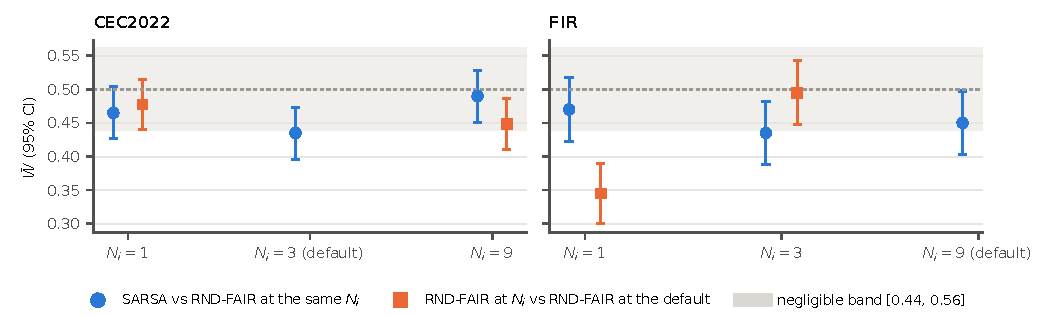
\includegraphics[width=0.85\textwidth]{figures/fig_dose.pdf}
\caption{Effect of the number of mediator episodes per subset member, $N_i$. Circles: SARSA vs RND-FAIR at the same $N_i$;
squares: RND-FAIR at $N_i$ vs RND-FAIR at the default $N_i$ of the benchmark.}
\label{fig:dose}
\end{figure}

\subsection{Study I: a check of the value-table properties}
\label{sec:theorycheck}
The propositions of Section~\ref{sec:theory} hold by construction; whether their consequences matter depends on the rewards
that the mediator produces. We logged every mediator episode of \res{A-th-runs} additional MPHBS runs (5 per instance, seeds
disjoint from the study): the reward, the provenance of the evaluated candidate's coordinates, and the table. For each cell
$(d,n,c)$ we computed the mean reward of the candidates whose coordinate $d$ was copied from rank $n$ of source $c$, which is
the quantity a useful table would have to rank (Table~\ref{tab:theory}). This check was not part of the pre-registration.

% generated by scripts/pathA_theory_assets.py -- do not edit
\begin{table*}[!t]
\centering
\caption{Post hoc check of Section~\ref{sec:theory} (5 runs per instance; medians over runs, interquartile ranges in
brackets). $p_+$: share of episodes with reward $+1$. $\sigma$: reward standard deviation. $\mathrm{sd}(Q)$: noise
standard deviation of a table entry predicted by Proposition~\ref{prop:noise}. $\hat\tau$: between-cell standard deviation
of the mean reward of the choices tried (method of moments, cells with at least 30 trials). $z$: separation of two
cells that differ by $\hat\tau$, Corollary~\ref{cor:order}. $\rho_{1/2}$: Spearman correlation of the cells' mean
rewards between the first and second half of the run. $\rho_Q$: Spearman correlation between the table at mid-run and
the cells' mean rewards in the second half.}
\label{tab:theory}
\footnotesize
\begin{tabular}{lcccccccc}
\toprule
Benchmark & runs & $p_+$ & $\sigma$ & $\mathrm{sd}(Q)$ & $\hat\tau$ & $z$ & $\rho_{1/2}$ & $\rho_Q$ \\
\midrule
CEC2022 ($D=20$) & 60 & 2.9\% & 0.35 & 0.094 & 0.045 & 0.58 & 0.57 [0.48, 0.66] & -0.39 [-0.46, -0.27] \\
FIR ($D=31$) & 40 & 12.5\% & 0.71 & 0.192 & 0.029 & 0.16 & 0.03 [0.00, 0.06] & 0.00 [-0.05, 0.04] \\
\bottomrule
\end{tabular}
\end{table*}


Rewards are sparse: \res{A-th-CEC-p_plus} of CEC2022 episodes and \res{A-th-FIR-p_plus} of FIR episodes improve on the current
vector, so almost every update is the rejected-candidate case of Propositions~\ref{prop:credit} and~\ref{prop:noise}. Between
cells, the mean reward of the choices tried differs by $\hat\tau=\res{A-th-CEC-tau_action}$ on CEC2022 and
$\res{A-th-FIR-tau_action}$ on FIR, which the noise floor turns into a separation of only $z=\res{A-th-CEC-z_typical}$ and
$\res{A-th-FIR-z_typical}$ (Corollary~\ref{cor:order}). The two benchmarks then differ. On FIR there is nothing stable to
learn: the cells' mean rewards in the two halves of a run are uncorrelated ($\rho_{1/2}=\res{A-th-FIR-split_half_rho}$), and so
is the table with later outcomes ($\rho_Q=\res{A-th-FIR-Qmid_validity_rho}$, positive in \res{A-th-FIR-valid-pos} of
\res{A-th-FIR-n} runs). On CEC2022 there is a stable signal ($\rho_{1/2}=\res{A-th-CEC-split_half_rho}$), but the table ranks
the cells against it: $\rho_Q=\res{A-th-CEC-Qmid_validity_rho}$, negative in all but \res{A-th-CEC-valid-pos} of
\res{A-th-CEC-n} runs. This is what Proposition~\ref{prop:credit} leads one to expect. A provenance that produces good vectors
keeps them current for many episodes, and in each of these episodes the table charges it with the failure of whatever
candidate is tried next; the better the provenance, the more penalties it collects. The noise floor would limit any table with
$\alpha=0.1$, while the credit assignment is specific to this mediator and would remain if $\alpha$ were changed.

\subsection{Study I: BBOB extension (exploratory)}
\label{sec:bbob}
To check whether L1 and L3 hold beyond the original two benchmark sets, SARSA, RND-FAIR and SKEL were run on the 24 BBOB
functions at $D=10$ and $D=20$ ($10{,}000D$ FEs, configuration B-C1, 30 paired runs per function; \res{A-bbob-runs} runs). At
$D=10$ SARSA and random assembly are practically equivalent ($\bar W=\res{A-bbob-B1-D10-wbar}$ \res{A-bbob-B1-D10-ci});
at $D=20$ the verdict is mixed (SARSA better on f3, random assembly on f9) and the interval for $\bar W$
(\res{A-bbob-B1-D20-wbar} \res{A-bbob-B1-D20-ci}) again lies below 0.5. The value of the mediator depends on the function
class (Table~\ref{tab:bbob-groups}): it helps strongly on separable or nearly separable functions and hurts on rotated,
ill-conditioned or non-separable ones such as f10, f12, f13 and f15, which matches its mechanism and motivates Study~II.

% generated by scripts/paper_bbob_assets.py -- do not edit
\begin{table*}[!t]
\centering
\caption{BBOB by function group: mean paired win probability of SARSA over the group's functions, and the number of
functions significant (Holm over all 24) in favour of SARSA / of the comparator.}
\label{tab:bbob-groups}
\footnotesize
\begin{tabular}{lcccc}
\toprule
 & \multicolumn{2}{c}{B1: SARSA vs RND-FAIR} & \multicolumn{2}{c}{B3: SARSA vs SKEL} \\
\cmidrule(lr){2-3}\cmidrule(lr){4-5}
Group & $D=10$ & $D=20$ & $D=10$ & $D=20$ \\
\midrule
separable (f1--f5) & 0.53 (0/0) & 0.54 (1/0) & 0.69 (2/0) & 0.70 (2/0) \\
low/moderate conditioning (f6--f9) & 0.45 (0/0) & 0.35 (0/1) & 0.50 (1/1) & 0.77 (2/0) \\
high conditioning (f10--f14) & 0.51 (0/0) & 0.40 (0/0) & 0.29 (0/2) & 0.49 (1/2) \\
multimodal, adequate structure (f15--f19) & 0.52 (0/0) & 0.41 (0/0) & 0.48 (0/2) & 0.46 (1/1) \\
multimodal, weak structure (f20--f24) & 0.49 (0/0) & 0.48 (0/0) & 0.40 (1/2) & 0.41 (1/3) \\
\bottomrule
\end{tabular}
\end{table*}


\subsection{Study II: the eigen-frame exchange}
\label{sec:resII}

\paragraph{Confirmatory tests (F1, F2)} On the 28 held-out instances, EIG-MPHBS is better than MPHBS-R on \res{E-H1-ngt}
instances, tied on \res{E-H1-neq} and worse on \res{E-H1-nlt} (one-sided $p=\res{E-H1-p}$), and better than MPHBS on
\res{E-H2-ngt}, tied on \res{E-H2-neq} and worse on \res{E-H2-nlt} ($p=\res{E-H2-p}$). After Holm correction both hypotheses
are supported ($p_\text{Holm}=\res{E-H1-pholm}$ for each; Table~\ref{tab:confirm}, Fig.~\ref{fig:heldout}). The evidence is
not strong: the median effects are small (\res{E-H1-medA} and \res{E-H2-medA}) because most CEC2022 $D=10$ functions are
solved equally well by all three variants, and when instances with $A=0.5$ are kept in the test with Pratt or zero-split
handling the Holm-adjusted $p$-values become \res{E-H1-pholm-pratt} and \res{E-H1-pholm-zsplit}. The rule fixed in advance
used the default handling; we report the alternatives so that readers can weigh the result. Per instance, EIG-MPHBS is
significantly better than MPHBS-R on \res{E-H1-sigfor} held-out instances (BBOB f6, f9, f11, f14, f19) and worse on
\res{E-H1-sigagainst} (f4, the separable Rastrigin variant); against MPHBS it is better on \res{E-H2-sigfor} and never
significantly worse. On all 56 instances the median $A$ is \res{E-S1-H1-medA} against MPHBS-R ($p=\res{E-S1-H1-p}$;
\res{E-S1-H1-sigfor} instances significantly better, \res{E-S1-H1-sigagainst} worse) and \res{E-S1-H2-medA} against MPHBS
($p=\res{E-S1-H2-p}$; \res{E-S1-H2-sigfor} better, \res{E-S1-H2-sigagainst} worse), with the largest effects on FIR (median
$A$ \res{E-S1-H2-FIR-medA}) and CEC2022 $D=20$ (\res{E-S1-H2-C20-medA}); these include the pilot instances on which $q$ was
chosen, so their effect sizes may be optimistic.

% generated by scripts/eswa_paper_assets.py -- do not edit
\begin{table}[!htbp]
\centering
\caption{Confirmatory tests on the 28 held-out instances (F1, F2) and their repetition on all 56 instances
(F1$'$, F2$'$, secondary: the 28 additional instances include those used to choose the eigen-frame probability).
$\tilde A$: median Vargha--Delaney effect over instances ($>0.5$ favours EIG-MPHBS). W/T/L: instances with
$A>0.5$, $A=0.5$, $A<0.5$. $p$: one-sided Wilcoxon signed-rank test of $A-0.5$ over instances; Holm over
\{F1, F2\}. The two sensitivity columns keep the instances with $A=0.5$ (Pratt and zero-split handling).
Sig.: instances where a paired per-instance test (Holm within benchmark) favours EIG-MPHBS / the comparator.}
\label{tab:confirm}
\footnotesize
\setlength{\tabcolsep}{4pt}
\resizebox{\textwidth}{!}{%
\begin{tabular}{llccccccc}
\toprule
 & Comparison & $\tilde A$ & W/T/L & $p$ & $p_\text{Holm}$ & $p_\text{Holm}$ (Pratt) & $p_\text{Holm}$ (zsplit) & Sig. \\
\midrule
F1 & EIG-MPHBS vs MPHBS-R & 0.500 & 14/6/8 & 0.031 & 0.043 & 0.056 & 0.057 & 5/1 \\
F2 & EIG-MPHBS vs MPHBS & 0.514 & 15/5/8 & 0.022 & 0.043 & 0.056 & 0.057 & 6/0 \\
\midrule
F1$'$ & all 56 instances (vs MPHBS-R) & 0.520 & 31/7/18 & \ensuremath{7.7{\times}10^{-4}} & -- & -- & -- & 12/1 \\
F2$'$ & all 56 instances (vs MPHBS) & 0.529 & 33/6/17 & \ensuremath{5.2{\times}10^{-4}} & -- & -- & -- & 14/0 \\
\bottomrule
\end{tabular}}
\end{table}


\begin{figure}[!htbp]
\centering
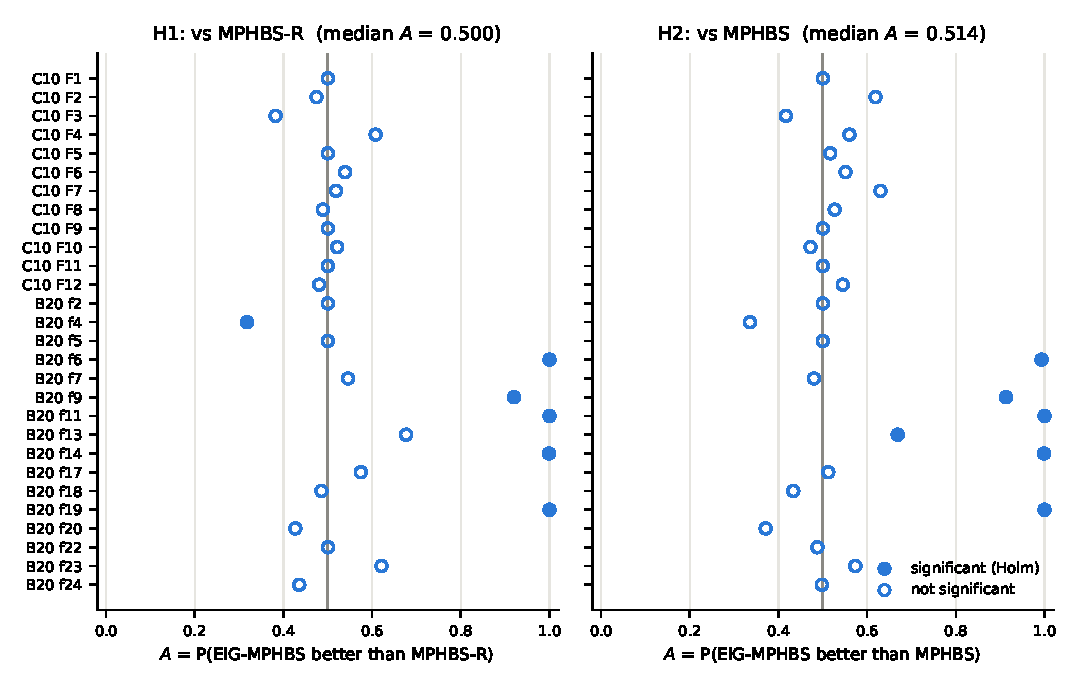
\includegraphics[width=\linewidth]{figures/fig_heldout.pdf}
\caption{Effect size $A$ of EIG-MPHBS on each of the 28 held-out instances against MPHBS-R (F1) and MPHBS (F2); $A>0.5$
favours EIG-MPHBS. Filled markers: significant per-instance paired test (Holm within benchmark). C10: CEC2022 $D=10$; B20:
BBOB $D=20$.}
\label{fig:heldout}
\end{figure}

\paragraph{Rotation dependence} Table~\ref{tab:rotation} compares BBOB functions that differ only by a rotation. On the
separable ellipsoid (f2) all algorithms reach the accuracy floor. On the rotated ellipsoid (f10), MPHBS and MPHBS-R stall at
median errors of \res{E-f10-MPHBS} and \res{E-f10-RND}, while EIG-MPHBS reaches \res{E-f10-EIG50}, a
\res{E-f10-ratio-RND}-fold reduction relative to MPHBS-R and \res{E-f10-ratio-MPHBS}-fold relative to MPHBS. On Rastrigin the
rotated version (f15) is hard for all three hybrids and the eigen frame does not help (median \res{E-f15-EIG50} against
\res{E-f15-RND} for MPHBS-R), and on the separable version (f3) EIG-MPHBS is slightly worse (\res{E-f3-EIG50} against
\res{E-f3-RND}), as expected when half of the exchanges no longer follow the axes along which the function separates. The gap
to CMA-ES and L-SHADE on f10 remains because Phase~1 is still coordinate-wise.

% generated by scripts/eswa_paper_assets.py -- do not edit
\begin{table}[!htbp]
\centering
\caption{Median final error on BBOB function pairs that differ only by a rotation ($D=20$, 30 runs; values at or
below $10^{-8}$ shown as 0).}
\label{tab:rotation}
\small
\begin{tabular}{lcccc}
\toprule
 & \multicolumn{2}{c}{Ellipsoid} & \multicolumn{2}{c}{Rastrigin} \\
\cmidrule(lr){2-3}\cmidrule(lr){4-5}
Algorithm & f2 (separable) & f10 (rotated) & f3 (separable) & f15 (rotated) \\
\midrule
EIG-MPHBS & 0 & 8.47 & 1.99 & 54.2 \\
MPHBS-R & 0 & 89.9 & 0.995 & 58.7 \\
MPHBS & 0 & 121 & 0.995 & 51.2 \\
CMA-ES & 0 & 0 & 8.95 & 2.98 \\
L-SHADE & 0 & 0 & 0 & 4.13 \\
\bottomrule
\end{tabular}
\end{table}


\paragraph{Mechanism} Fig.~\ref{fig:mechanism} shows the fraction of exchanged candidates that are accepted in each iteration
and the diversity of the populations. On the rotated ellipsoid f10 the axis-frame exchange almost stops working after the first
few thousand evaluations: in the first quarter of the budget \res{E-acc-B20-10-RND}\% of the candidates of MPHBS-R and
\res{E-acc-B20-10-MPHBS}\% of those of MPHBS are accepted, against \res{E-acc-B20-10-EIG50}\% for EIG-MPHBS; the discus f11
shows the same pattern (\res{E-acc-B20-11-RND}\% and \res{E-acc-B20-11-MPHBS}\% against \res{E-acc-B20-11-EIG50}\%). Because
the candidates stay inside the valley, the populations contract faster along it. This supports the explanation of
Section~\ref{sec:eigen}: the frame restores the exchange channel on coupled problems rather than changing the native moves.

\begin{figure}[!htbp]
\centering
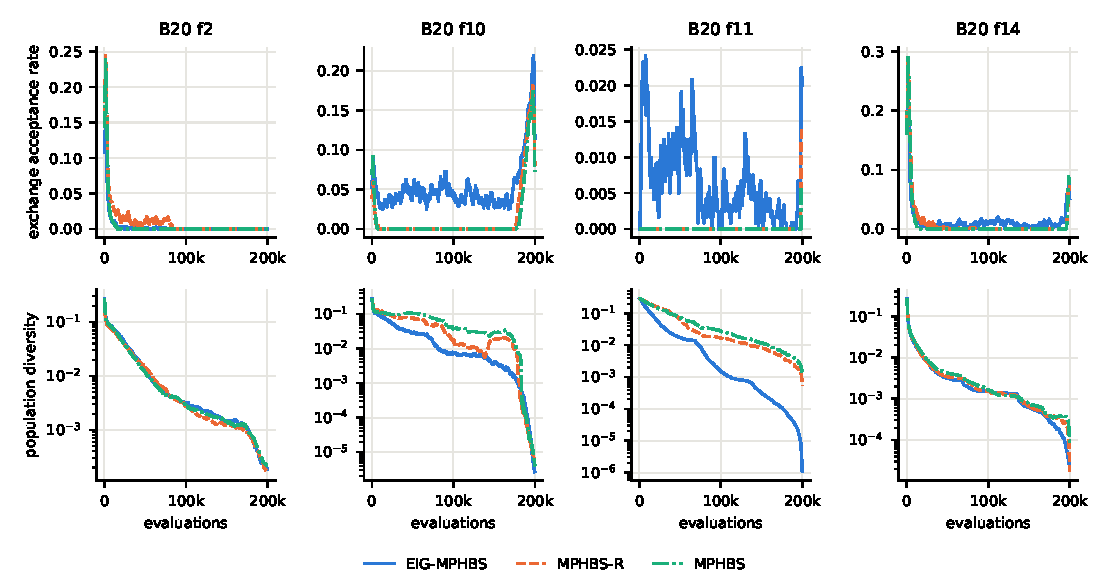
\includegraphics[width=\textwidth]{figures/fig_mechanism.pdf}
\caption{Mechanism of the eigen frame on BBOB $D=20$. Top: fraction of exchanged candidates accepted per iteration (moving
average over 25 iterations). Bottom: population diversity (log scale). Medians over 30 runs. f2 is separable; f10, f11 and f14
are rotated.}
\label{fig:mechanism}
\end{figure}

\paragraph{Comparison with ten algorithms} Fig.~\ref{fig:ranks} and Table~\ref{tab:ranks} give the mean Friedman
ranks~\citep{derrac2011tutorial} of the eleven algorithms and Table~\ref{tab:wtl} the per-instance significance of
EIG-MPHBS against each. EIG-MPHBS ranks \res{E-pos-EIG50} of 11 overall (mean rank \res{E-rank-EIG50}), behind L-SHADE
(\res{E-rank-L-SHADE}) and CMA-ES (\res{E-rank-CMA-ES}) and ahead of MPHBS-R (\res{E-rank-RND}), MPHBS (\res{E-rank-MPHBS}) and
all classical metaheuristics. It is significantly better than MPHBS on \res{E-win-MPHBS} instances and worse on none, better
than MPHBS-R on \res{E-win-RND} and worse on \res{E-loss-RND}, better than HBA on \res{E-win-HBA} of 56 and worse on none, and
better than MPA on \res{E-win-MPA} and worse on \res{E-loss-MPA}. Over PSO, DE, GWO and WOA it wins \res{E-common-win} and
loses \res{E-common-loss} of \res{E-common-n} comparisons; GWO and WOA are known to be biased towards the centre of the search
space~\citep{kudela2022centre}. L-SHADE and CMA-ES are clearly stronger at $D=20$, on BBOB and on FIR.

\begin{figure}[!htbp]
\centering
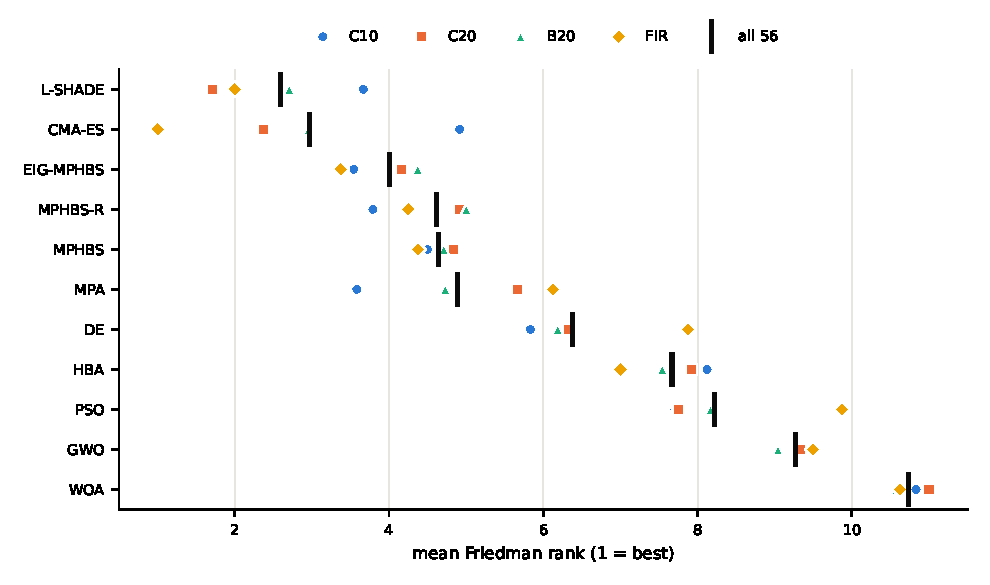
\includegraphics[width=0.92\linewidth]{figures/fig_ranks.pdf}
\caption{Mean Friedman rank of each algorithm per benchmark (markers) and over all 56 instances (vertical bar); 1 = best.
C10/C20: CEC2022 $D=10/20$; B20: BBOB $D=20$.}
\label{fig:ranks}
\end{figure}

% generated by scripts/eswa_paper_assets.py -- do not edit
\begin{table}[!htbp]
\centering
\caption{Mean Friedman rank of the eleven algorithms (rank of the median final error on each instance, 1 = best;
lowest in bold), per benchmark and over all 56 instances. Last row: Friedman test $p$ per benchmark.}
\label{tab:ranks}
\small
\begin{tabular}{lccccc}
\toprule
Algorithm & C10 & C20 & B20 & FIR & All \\
 & (12) & (12) & (24) & (8) & (56) \\
\midrule
L-SHADE & 3.67 & \textbf{1.71} & \textbf{2.71} & 2.00 & \textbf{2.60} \\
CMA-ES & 4.92 & 2.38 & 2.96 & \textbf{1.00} & 2.97 \\
EIG-MPHBS & \textbf{3.54} & 4.17 & 4.38 & 3.38 & 4.01 \\
MPHBS-R & 3.79 & 4.92 & 5.00 & 4.25 & 4.62 \\
MPHBS & 4.50 & 4.83 & 4.71 & 4.38 & 4.64 \\
MPA & 3.58 & 5.67 & 4.73 & 6.12 & 4.88 \\
DE & 5.83 & 6.33 & 6.19 & 7.88 & 6.38 \\
HBA & 8.12 & 7.92 & 7.54 & 7.00 & 7.67 \\
PSO & 7.71 & 7.75 & 8.17 & 9.88 & 8.22 \\
GWO & 9.50 & 9.33 & 9.04 & 9.50 & 9.27 \\
WOA & 10.83 & 11.00 & 10.58 & 10.62 & 10.73 \\
\midrule
Friedman $p$ & \ensuremath{3.9{\times}10^{-14}} & \ensuremath{1.3{\times}10^{-14}} & \ensuremath{2.8{\times}10^{-26}} & \ensuremath{1.4{\times}10^{-12}} & -- \\
\bottomrule
\end{tabular}
\end{table}

% generated by scripts/eswa_paper_assets.py -- do not edit
\begin{table}[!htbp]
\centering
\caption{EIG-MPHBS against each algorithm: number of instances where it is significantly better / not
significantly different / significantly worse (paired two-sided Wilcoxon signed-rank test over the 30 seed-paired
runs, Holm within each benchmark and comparator, $\alpha=0.05$).}
\label{tab:wtl}
\small
\begin{tabular}{lccccc}
\toprule
vs & C10 (12) & C20 (12) & B20 (24) & FIR (8) & Total (56) \\
\midrule
L-SHADE & 1/9/2 & 0/4/8 & 3/5/16 & 0/0/8 & 4/18/34 \\
CMA-ES & 3/7/2 & 1/5/6 & 4/5/15 & 0/0/8 & 8/17/31 \\
MPHBS-R & 0/12/0 & 3/9/0 & 7/16/1 & 2/6/0 & 12/43/1 \\
MPHBS & 0/12/0 & 2/10/0 & 7/17/0 & 5/3/0 & 14/42/0 \\
MPA & 1/11/0 & 5/5/2 & 10/10/4 & 8/0/0 & 24/26/6 \\
DE & 9/2/1 & 7/3/2 & 13/8/3 & 8/0/0 & 37/13/6 \\
HBA & 10/2/0 & 10/2/0 & 19/5/0 & 8/0/0 & 47/9/0 \\
PSO & 9/3/0 & 9/3/0 & 18/5/1 & 8/0/0 & 44/11/1 \\
GWO & 12/0/0 & 12/0/0 & 20/4/0 & 8/0/0 & 52/4/0 \\
WOA & 12/0/0 & 12/0/0 & 24/0/0 & 8/0/0 & 56/0/0 \\
\bottomrule
\end{tabular}
\end{table}


\paragraph{Comparison with EA4eig and cost} EA4eig~\citep{bujok2022ea4eig}, which combines eigen crossover with four strong
algorithms, is significantly better than EIG-MPHBS on \res{E-ea4eig-D10-worse} of 12 CEC2022 functions at $D=10$ and
\res{E-ea4eig-D20-worse} of 12 at $D=20$ at the competition budgets (official results; unpaired, descriptive;
Table~\ref{tab:ea4eig}), and EIG-MPHBS is never significantly better. The eigen frame adds
\res{E-overhead-min}--\res{E-overhead-max}\% to the median run time of MPHBS-R, and EIG-MPHBS is faster than MPHBS, whose
SARSA bookkeeping costs more than the decomposition (Table~\ref{tab:cost}).

% generated by scripts/eswa_paper_assets.py -- do not edit
\begin{table}[!htbp]
\centering
\caption{EIG-MPHBS against the official CEC2022 runs of EA4eig at the competition budgets ($2\times10^5$
evaluations for $D=10$, $10^6$ for $D=20$; 30 runs each). Median final error (at or below $10^{-8}$ shown as 0) and
Vargha--Delaney $A$ ($>0.5$ favours EIG-MPHBS). Superscripts: two-sided Mann--Whitney test, Holm over the 12
functions of each dimension ($^{+}$ EIG-MPHBS better, $^{-}$ worse, $^{\approx}$ no significant difference).
Unpaired and descriptive: hardware and implementation differ.}
\label{tab:ea4eig}
\small
\begin{tabular}{lcccccc}
\toprule
 & \multicolumn{3}{c}{$D=10$} & \multicolumn{3}{c}{$D=20$} \\
\cmidrule(lr){2-4}\cmidrule(lr){5-7}
 & EIG-MPHBS & EA4eig & $A$ & EIG-MPHBS & EA4eig & $A$ \\
\midrule
F1 & 0$^{\approx}$ & 0 & 0.50 & 0$^{\approx}$ & 0 & 0.50 \\
F2 & 0$^{\approx}$ & 0 & 0.46 & 47$^{-}$ & 0 & 0.17 \\
F3 & 2.27e-7$^{-}$ & 0 & 0.13 & 7.77e-8$^{-}$ & 0 & 0.15 \\
F4 & 7.96$^{-}$ & 0.995 & 0.01 & 34.8$^{-}$ & 6.96 & 0.00 \\
F5 & 0$^{\approx}$ & 0 & 0.50 & 14.1$^{-}$ & 0 & 0.00 \\
F6 & 0.155$^{-}$ & 5.41e-3 & 0.04 & 3.28$^{-}$ & 0.106 & 0.01 \\
F7 & 2.36e-6$^{-}$ & 0 & 0.02 & 25.3$^{-}$ & 2.3 & 0.03 \\
F8 & 0.16$^{-}$ & 0.0467 & 0.27 & 20.6$^{-}$ & 20.3 & 0.29 \\
F9 & 229$^{-}$ & 186 & 0.00 & 181$^{-}$ & 165 & 0.00 \\
F10 & 100$^{-}$ & 100 & 0.11 & 100$^{\approx}$ & 100 & 0.34 \\
F11 & 0$^{\approx}$ & 0 & 0.50 & 300$^{-}$ & 300 & 0.16 \\
F12 & 159$^{-}$ & 146 & 0.00 & 240$^{-}$ & 200 & 0.00 \\
\bottomrule
\end{tabular}
\end{table}

% generated by scripts/eswa_paper_assets.py -- do not edit
\begin{table}[!htbp]
\centering
\caption{Median wall-clock time per run in seconds (Python 3, NumPy, one core per run, 11 runs in parallel on a
12-core laptop; other jobs shared the machine, so times are indicative). Last row: median paired ratio of the run
times of EIG-MPHBS and MPHBS-R, which use identical evaluation counts.}
\label{tab:cost}
\small
\begin{tabular}{lcccc}
\toprule
Algorithm & C10 & C20 & B20 & FIR \\
\midrule
EIG-MPHBS & 61.3 & 60.9 & 133.2 & 79.8 \\
MPHBS-R & 60.6 & 59.2 & 132.1 & 77.1 \\
MPHBS & 81.1 & 75.9 & 158.3 & 86.9 \\
HBA & 7.1 & 8.4 & 8.4 & 20.5 \\
MPA & 4.5 & 5.7 & 5.7 & 19.2 \\
L-SHADE & 19.4 & 11.6 & 23.4 & 24.9 \\
CMA-ES & 120.8 & 89.1 & 183.2 & 75.6 \\
DE & 17.6 & 18.2 & 18.3 & 28.4 \\
PSO & 4.9 & 6.1 & 5.9 & 19.3 \\
GWO & 5.7 & 7.2 & 7.0 & 18.9 \\
WOA & 5.5 & 6.6 & 6.4 & 17.7 \\
\midrule
EIG-MPHBS / MPHBS-R & 1.055 & 1.033 & 1.032 & 1.032 \\
\bottomrule
\end{tabular}
\end{table}


\paragraph{Frame probability} \label{sec:ablation} Table~\ref{tab:ablation} reports the 10-run pilot that preceded the
confirmatory runs: four variants on 28 instances. Removing the exchange altogether is clearly harmful on FIR and CEC2022
$D=20$; $q=0.5$ has the best mean rank on CEC2022 $D=20$ and FIR and ties with $q=1$ on the eight BBOB pilot instances;
always using the eigen frame loses some of the benefit on FIR, which has partly separable structure. With 10 runs few
per-instance differences are significant, so the table supports the choice of $q=0.5$ but does not show that it is optimal.

% generated by scripts/eswa_paper_assets.py -- do not edit
\begin{table}[!htbp]
\centering
\caption{Ablation and sensitivity to the eigen-frame probability $q$ in the pilot study (10 seed-paired runs per
instance; exploratory, and these instances are excluded from the confirmatory test). ``No exchange'' removes Phase 2;
$q=0$ is MPHBS-R; $q=0.5$ is EIG-MPHBS; $q=1$ always uses the eigen frame. Left: mean rank of the median final error
(1 = best). Right: median Vargha--Delaney $A$ of $q=0.5$ against $q=0$ and $q=1$, with the number of instances where it
is significantly better / not different / worse (paired Wilcoxon, Holm within benchmark). $^\ast$BBOB f1, f3, f8, f10,
f12, f15, f16, f21.}
\label{tab:ablation}
\small
\begin{tabular}{lcccccc}
\toprule
 & \multicolumn{4}{c}{Mean rank} & \multicolumn{2}{c}{$q=0.5$ against} \\
\cmidrule(lr){2-5}\cmidrule(lr){6-7}
Benchmark & no exchange & $q=0$ & $q=0.5$ & $q=1$ & $q=0$ & $q=1$ \\
\midrule
B20$^\ast$ (8) & 2.19 & 2.94 & 2.44 & 2.44 & 0.51 (2/6/0) & 0.47 (1/7/0) \\
C20 (12) & 2.67 & 2.92 & 1.88 & 2.54 & 0.64 (1/11/0) & 0.61 (1/11/0) \\
FIR (8) & 4.00 & 2.25 & 1.38 & 2.38 & 0.65 (1/7/0) & 0.69 (1/7/0) \\
\bottomrule
\end{tabular}
\end{table}


\subsection{Study III: transfer to other parent pairs}
\label{sec:resIII}
All \res{X-runs} runs of Study~III completed with identical FE counts for each eigen arm and its axis twin. Table~\ref{tab:transfer}
and Fig.~\ref{fig:transfer} give the confirmatory test T1.

% generated by scripts/combined_assets.py -- do not edit
\begin{table}[!htbp]
\centering
\caption{Transfer of the eigen-frame exchange to two other parent pairs (T1): eigen-frame arm against its axis-frame twin,
32 instances, 30 seed-paired runs per instance and arm. $\tilde A$: median Vargha--Delaney effect over instances ($>0.5$
favours the eigen frame); W/T/L: instances with $A>0.5$, $A=0.5$, $A<0.5$; $p$: one-sided Wilcoxon signed-rank test of
$A-0.5$; $p_\text{Holm}$: Holm over the two pairs; the next column gives $p$ with Pratt and zero-split handling of
$A=0.5$ (before Holm). Sig.: instances where a paired per-instance test (Holm within benchmark and pair) favours the
eigen frame / the axis frame.}
\label{tab:transfer}
\footnotesize
\setlength{\tabcolsep}{4pt}
\begin{tabular}{lcccccc}
\toprule
Parent pair & $\tilde A$ & W/T/L & $p$ & $p_\text{Holm}$ & $p$ (Pratt / zsplit) & Sig. \\
\midrule
PSO + DE & \res{X-PD-medA} & \res{X-PD-ngt}/\res{X-PD-neq}/\res{X-PD-nlt} & \res{X-PD-p} & \res{X-PD-pholm} & \res{X-PD-ppratt} / \res{X-PD-pzsplit} & \res{X-PD-sige}/\res{X-PD-siga} \\
\quad BBOB $D=20$ (24) & \res{X-PD-B20-medA} & & & & & \res{X-PD-B20-sige}/\res{X-PD-B20-siga} \\
\quad FIR (8) & \res{X-PD-FIR-medA} & & & & & \res{X-PD-FIR-sige}/\res{X-PD-FIR-siga} \\
\midrule
GWO + WOA & \res{X-GW-medA} & \res{X-GW-ngt}/\res{X-GW-neq}/\res{X-GW-nlt} & \res{X-GW-p} & \res{X-GW-pholm} & \res{X-GW-ppratt} / \res{X-GW-pzsplit} & \res{X-GW-sige}/\res{X-GW-siga} \\
\quad BBOB $D=20$ (24) & \res{X-GW-B20-medA} & & & & & \res{X-GW-B20-sige}/\res{X-GW-B20-siga} \\
\quad FIR (8) & \res{X-GW-FIR-medA} & & & & & \res{X-GW-FIR-sige}/\res{X-GW-FIR-siga} \\
\bottomrule
\end{tabular}
\end{table}


\begin{figure}[!htbp]
\centering
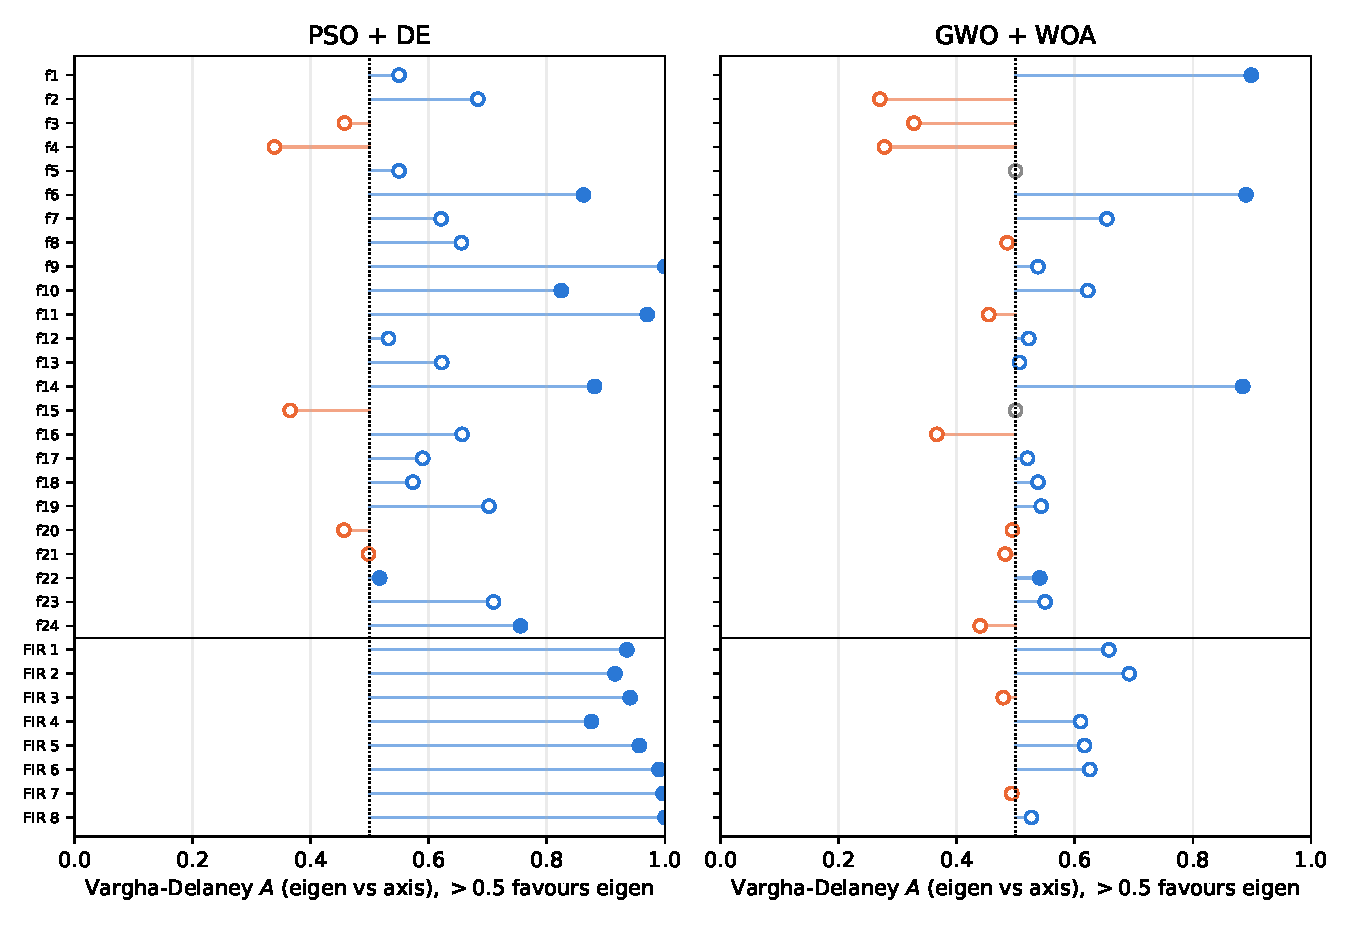
\includegraphics[width=\textwidth]{figures/fig_transfer.pdf}
\caption{Study III: Vargha--Delaney effect $A$ of the eigen-frame arm against its axis-frame twin on the 32 instances for each
parent pair. $A>0.5$ favours the eigen frame (blue); filled markers: significant per-instance paired test (Holm within
benchmark and pair). The horizontal line separates BBOB $D=20$ (top) from FIR.}
\label{fig:transfer}
\end{figure}

\paragraph{PSO with DE} The eigen frame outperforms the axis frame: the median $A$ is \res{X-PD-medA}, better on \res{X-PD-ngt}
and worse on \res{X-PD-nlt} of \res{X-PD-n} instances ($p=\res{X-PD-p}$, $p_\text{Holm}=\res{X-PD-pholm}$), and the result does
not depend on the handling of ties ($p=\res{X-PD-ppratt}$ and \res{X-PD-pzsplit} with Pratt and zero-split handling). It is
significantly better on \res{X-PD-sige} instances and significantly worse on \res{X-PD-siga}: \res{X-PD-B20-sige} of 24 on BBOB
(median $A$ \res{X-PD-B20-medA}) and all \res{X-PD-FIR-sige} of 8 on FIR (median $A$ \res{X-PD-FIR-medA}).

\paragraph{GWO with WOA} The hypothesis is supported, but narrowly and with a small effect: the median $A$ is \res{X-GW-medA},
better on \res{X-GW-ngt}, tied on \res{X-GW-neq} and worse on \res{X-GW-nlt} instances ($p=\res{X-GW-p}$, $p_\text{Holm}=
\res{X-GW-pholm}$; Pratt and zero-split handling give \res{X-GW-ppratt} and \res{X-GW-pzsplit} before Holm). The eigen frame is
significantly better on \res{X-GW-sige} instances, all on BBOB (median $A$ \res{X-GW-B20-medA}), and significantly worse on
none; on FIR the median $A$ is \res{X-GW-FIR-medA} with no significant instance. We read this as a small effect in a
consistent direction, not as a general gain.

\paragraph{Rotation and mechanism} On the rotated ellipsoid f10 the median error falls from \res{X-ell-rot-PDR} to
\res{X-ell-rot-PDE} for PSO with DE and from \res{X-ell-rot-GWR} to \res{X-ell-rot-GWE} for GWO with WOA, while both pairs reach
(PSO+DE) or approach (GWO+WOA) the floor on the separable f2 in either frame, as in Study~II. On rotated Rastrigin f15 the eigen
frame does not help PSO with DE (\res{X-ras-rot-PDE} against \res{X-ras-rot-PDR}) and is on a par for GWO with WOA
(\res{X-ras-rot-GWE} against \res{X-ras-rot-GWR}), and on the separable f3 it is worse for PSO with DE (\res{X-ras-sep-PDE} against \res{X-ras-sep-PDR}), the
same pattern as in Study~II. The acceptance rate of exchanged candidates in the first quarter of the budget does \emph{not}
explain the gain in these pairs: on f10 it is \res{X-acc-PDE-f10}\% for the eigen arm against \res{X-acc-PDR-f10}\% for the axis
arm with PSO and DE, and \res{X-acc-GWE-f10}\% against \res{X-acc-GWR-f10}\% with GWO and WOA, so the higher acceptance seen
for the HBA--MPA hybrid (Study~II) is not a general mechanism. Why the frame helps PSO with DE is therefore not established by
these data.

%% =====================================================================
\section{Discussion}
\label{sec:discussion}

\paragraph{What drives the hybrid} Three components carry the performance of MPHBS on these benchmarks: exchanging
information between the populations at all (decisive on FIR), the amount of exchange per iteration, and the way the
population memory interacts with the mediator. The learned controller and the restructured loop are not among them.
Proposition~\ref{prop:credit} and~\ref{prop:noise} give the main reasons why learning does not help. The table has
$D\cdot N_\mathrm{sub}\cdot 2$ entries (320 on CEC2022, 496 on FIR) and receives $b=\lceil D/5\rceil$ updates per episode,
but by Proposition~\ref{prop:credit} only the provenance of the current vector is updated, so the median updated entry
receives \res{A-th-CEC-median_updates_per_updated_cell} updates on CEC2022 and every entry averages over only about
\res{A-th-memory} of them. The reward is the sign of the change of a whole assembled vector, shared by all $b$ dimensions of
the block, and the evaluated candidate was itself chosen by the proxy score from $K$ candidates generated by different
policies. Finally, the most informative choices, taking coordinates from good members, are already enforced by the ranked
subsets and the rank term of the proxy score~\eqref{eq:proxy}. These properties follow from the update rule and the
reward, not from the algorithm pair; they apply to any mediator of this form.

\paragraph{What carries the exchange} The exchange step is where the populations combine their information, and it was
written for separable problems. Moving it into the eigen frame of the pooled populations makes it invariant to rotations at
no evaluation cost, and Studies~II and~III show that the gain is not specific to one pair: it is large for PSO with DE and the
HBA--MPA hybrid, and small for GWO with WOA, for which these data give no explanation. The
frame helps unimodal or moderately multimodal problems with coupled variables, where the population covariance reflects the
basin; it does not help highly multimodal rotated functions such as f15, and it costs a little on separable multimodal ones
such as f3 and f4. Phase~1 remains coordinate-wise, which is why the gap to CMA-ES, L-SHADE and EA4eig on rotated functions
persists. This is an improvement of a hybrid within its class, not a new state of the art.

\paragraph{Matched controls} The re-evaluating control illustrates two ways in which a control can differ from the learned variant
without anybody intending it: a different number of iterations at the same budget, and a different update of a state
variable. Proposition~\ref{prop:identify} makes the requirement explicit, and Algorithm~\ref{alg:protocol} turns it into a
procedure whose budget and state checks would have exposed both differences before the first run. A paired, seed-matched
design also detects extremely consistent but tiny effects (L4); effect magnitudes should accompany consistency measures.

\paragraph{Practical guidance} For practitioners who use hybrids of this kind, the value table can be replaced by uniform
choices of source and rank without loss, the number of episodes is a more important parameter than the controller, the
treatment of the population memory deserves to be a deliberate decision, and the eigen-frame exchange is a drop-in
replacement with the same budget and a few percent of extra run time. When the choice of algorithm is open, L-SHADE and
CMA-ES remain the stronger default on problems of this size.

\subsection{Limitations}
\begin{itemize}
\item \emph{Scope.} Study~I covers one hybrid in its reference configurations, selected with SARSA on CEC2022 and FIR,
which makes L1 conservative; Studies~II and~III cover problems with $D\le31$. The confirmatory effect in Study~II is small and
sensitive to the handling of tied instances. No free lunch results~\citep{wolpert1997nfl} caution against generalising beyond the
problems studied.
\item \emph{Transfer.} Study~III covers two further pairs on two benchmark families with the mediator settings of the
reference hybrid; the effect for GWO with WOA is small, and the mechanism of the gain for PSO with DE is not identified.
\item \emph{Choices fixed by pilot.} The value $q=0.5$ was chosen from a pilot with two values; other values or an adaptive
$q$ may perform differently. The classical algorithms were added after the main analysis of Study~II and use standard, not
tuned, settings. The EA4eig comparison is unpaired and across implementations; run times were measured on a shared laptop.
\item \emph{Port and platform.} Study~I uses a Python port whose agreement with the reference MATLAB implementation is
distributional, because random streams differ.
\item \emph{Exploratory parts.} L5--L8, the theory check and the BBOB extension are exploratory and should be confirmed
independently. The relative difference $\hat\delta$ was added after the pre-registration.
\item \emph{Dimension.} For larger $D$ the $O(D^3)$ decomposition and the reliability of the covariance estimate from $2N$
points should be checked.
\end{itemize}

%% =====================================================================
\section{Conclusion}
\label{sec:conclusion}
A contrast between a learned component and a control mixes learning, budget and state effects unless the control is matched,
and ablations of learned components in metaheuristics should therefore be budget- and state-matched, verified mechanically,
fixed in advance and reported with effect magnitudes. In the hybrid studied here, random choices are as effective as the
learned controller at an equal budget; the update rule explains why, because it credits each reward to the provenance of the
current vector and its learning rate limits each entry to an average over about \res{A-th-memory} updates, and logged runs
confirm both effects. The exchange step carries the performance, and making it independent of the coordinate system, by
recombining in the eigenvector frame of the pooled populations, improves the hybrid without extra evaluations: in
\res{E-runs-total} runs on CEC2022, BBOB and FIR it was never significantly worse than the original and reduced the median
error on the rotated ellipsoid \res{E-f10-ratio-MPHBS}-fold. In a pre-registered study of \res{X-runs} runs the same exchange
helps two other parent pairs, strongly for PSO with DE and slightly for GWO with WOA. The remaining gap to CMA-ES, L-SHADE and
EA4eig, the failure on rotated multimodal functions and the missing mechanism for the transfer are the natural next steps,
together with an adaptive frame probability and rotation-invariant native moves.

\FloatBarrier
\section*{Statements and Declarations}
\paragraph{Competing interests} The author has no competing interests to declare that are relevant to the content of this article.
\paragraph{Funding} No funding was received for conducting this study.
\paragraph{Data and code availability} The repository \url{https://github.com/abinaya-g/la-kaie} holds the code, the frozen
pre-registrations and design documents (Study~I: tag \texttt{pathA-prereg-frozen} and the BBOB addendum, tag
\texttt{pathA-bbob-run-1}; Studies~II and~III: \path{experiments/ESWA_EIGEN_CAMPAIGN.md}, Sections 1--10), the record of every
run (final error, evaluations, run time, configuration and seed), the analyses and the scripts from which each number, table
and figure of this paper is produced (\path{scripts/combined_assets.py}). The official EA4eig results are redistributed with
their source in \path{data/external/cec2022_ea4eig/}.
\paragraph{Author contributions} Abinaya G conceived and designed the study, wrote the software, ran the experiments and the
analysis, and wrote the manuscript.
